\documentclass[11pt,tikz]{standalone}
\usepackage[T1]{fontenc}
\usepackage{amssymb}
\usepackage{amsthm}
\usepackage{tikz}
\usepackage{pgfplots}
\pgfplotsset{compat=1.18}
\usetikzlibrary{intersections,calc}
\begin{document}
	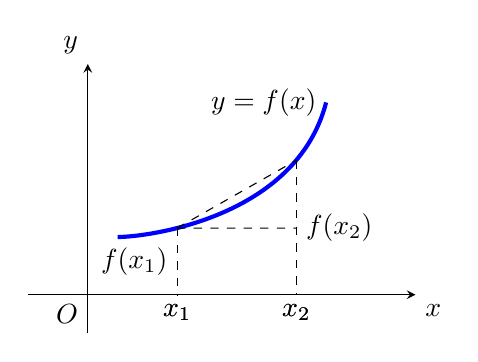
\begin{tikzpicture}[baseline={(0,0)}]
		\begin{axis}[
			clip=false,
			width=6.5cm, height=5cm,
			xmin=-1, xmax=5.5, ymin=-1, ymax=6,
			xtick=\empty, ytick=\empty,
			axis lines=middle, axis line style={->},
			xlabel={$x$}, ylabel={$y$},
			xlabel style={below right}, ylabel style={above left},
			>=stealth,
			]
			\draw[name path =curve,line width=1.5pt,color=blue] 
			(0.5,1.5) .. controls (1,1.5) and (3.5,2) .. (4,5);
			\path [name path =a_1] (1.5,0) -- (1.5,5);
			\path [name path = b_1] (3.5,0) -- (3.5,5);
			\path [name intersections={of =curve and a_1,by=a}]  ;
			\path [name intersections={of =curve and b_1,by=b}]  ;
			\draw[dashed] (a) -- (a |- 0,0)node[below]{$x_1$};
			\draw[dashed] (b) -- (b |- 0,0)node[below]{$x_2$};
			\draw [dashed] (a) -|(a -| b) (a) -- (b);
			\node[below] at (1.5,0) {$x_1$};
			\node[below] at (3.5,0) {$x_2$};
			\node[left] at ($(a)!0.5!(a |- 0,0)$) {$f(x_1)$};
			\node[right] at ($(b)!0.5!(b |- 0,0)$) {$f(x_2)$};
			\node[left] at (4,5) {$y=f(x)$};
			\node[below left] at (0,0) {$O$};
		\end{axis}
	\end{tikzpicture}
	
			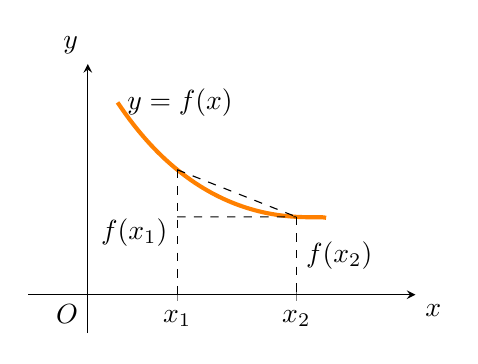
\begin{tikzpicture}[baseline={(0,0)}]
		\begin{axis}[
			clip=false,
			width=6.5cm, height=5cm,
			xmin=-1, xmax=5.5, ymin=-1, ymax=6,
			xtick=\empty, ytick=\empty,
			axis lines=middle, axis line style={->},
			xlabel={$x$}, ylabel={$y$},
			xlabel style={below right},
			ylabel style={above left},
			xtick={1.5,3.5},
			xticklabels={$x_1$,$x_2$},
			>=stealth,
			]
			\draw[name path=curve,line width=1.5pt,color=orange]%
				(0.5,5) .. controls (2,1.5) and (3.8,2.1) .. (4,2);
			\path [name path =a_1] (1.5,0) -- (1.5,5);
			\path [name path = b_1] (3.5,0) -- (3.5,5);
			\path [name intersections={of =curve and a_1,by=a}]  ;
			\path [name intersections={of =curve and b_1,by=b}]  ;
			\draw[dashed] (a) -- (a |- 0,0);
			\draw[dashed] (b) -- (b |- 0,0);
			\draw [dashed] (a |- b) -- (b) (a) -- (b);
			\node[left] at ($(a)!0.5!(a |- 0,0)$) {$f(x_1)$};
			\node[right] at ($(b)!0.5!(b |- 0,0)$) {$f(x_2)$};
			\node[right] at (0.5,5) {$y=f(x)$};
			\node[below left] at (0,0) {$O$};
		\end{axis}
	\end{tikzpicture}
	
			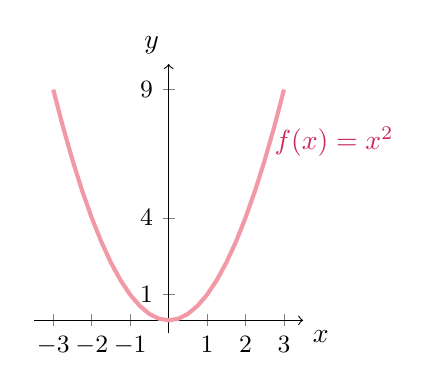
\begin{tikzpicture}[baseline=3cm]
		\begin{axis}[
			clip=false,
			width=5cm, height=5cm,
			xmin=-3.5, xmax=3.5,
			ymin=-0.5, ymax=10,
			xtick={-3,-2,-1,0,1,2,3},
			ytick={1,4,9},
			axis lines=middle,
			axis line style={->},
			xlabel={$x$}, ylabel={$y$},         
			xlabel style={below right},
			ylabel style={above left},
			tick label style={font=\small},
			]
			\addplot[color=pink!80!purple, line width=1.5pt, domain=-3:3] {x^2};
			\node[above right, pink!20!purple] at (2.5, 6) {$f(x)=x^2$};
		\end{axis}
	\end{tikzpicture}
	
		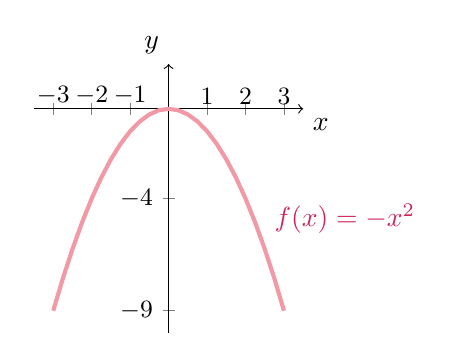
\begin{tikzpicture}[baseline=3cm]
		\begin{axis}[
			clip=false,
			width=5cm, height=5cm,
			xmin=-3.5, xmax=3.5,
			ymin=-10, ymax=2,
			xtick={-3,-2,-1,0,1,2,3},
			ytick={-4,-9},
			xticklabel style={above},
			axis lines=middle,
			axis line style={->},
			xlabel={$x$}, ylabel={$y$},
			xlabel style={below right},
			ylabel style={above left},
			tick label style={font=\small},
			]
			\addplot[color=pink!80!purple, line width=1.5pt, domain=-3:3] {-x^2};
			\node[above right, pink!20!purple] at (2.5, -6) {$f(x)=-x^2$};
		\end{axis}
	\end{tikzpicture}
	
			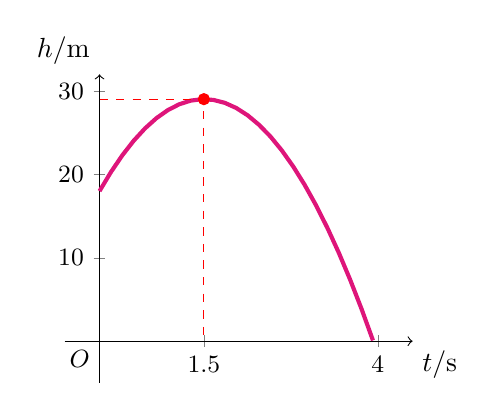
\begin{tikzpicture}[baseline=(current bounding box.north)]
		\begin{axis}[
			width=6cm, height=5.5cm,
			xmin=-0.5, xmax=4.5, ymin=-5, ymax=32,
			xtick={1.5,4},
			ytick={10,20,30},
			axis lines=middle, axis line style={->},
			xlabel={$t$/s}, ylabel={$h$/m},
			xlabel style={below right}, 
			ylabel style={above left},
			tick label style={font=\small},
			]
			\addplot[color=magenta!70!purple, line width=1.5pt, domain=0:3.93] {-4.9*x^2+14.7*x+18};
			\addplot[only marks, mark=*, mark size=2pt, color=red] coordinates {(1.5,29.025)};
			\draw[dashed, red] (0,29.025) -- (1.5,29.025) -- (1.5,0);
			\node[below left] at (axis cs:0,0) {\small$O$};
		\end{axis}
	\end{tikzpicture}
	
			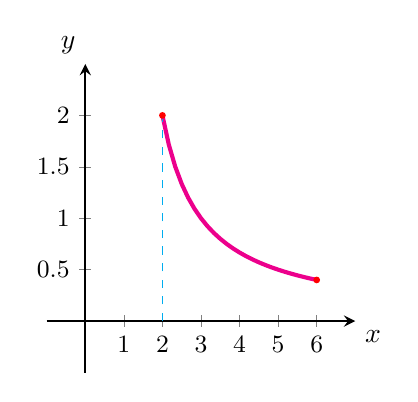
\begin{tikzpicture}[baseline=(current bounding box.north)]
		\begin{axis}[
			width=5.5cm, height=5.5cm,
			xmin=-1, xmax=7, ymin=-0.5, ymax=2.5,
			xtick={1,2,3,4,5,6},
			ytick={0.5,1,1.5,2},
			axis lines=middle, 
			axis line style={-stealth},
			xlabel={$x$}, ylabel={$y$},
			xlabel style={below right}, ylabel style={above left},
			tick label style={font=\small},
			axis line style={thick},
			]
			\addplot[magenta, line width=1.5pt, domain=2:6] {2/(x-1)};
			\addplot[only marks, mark=*, mark size=1pt, color=red] coordinates {(2,2) (6,0.4)};
			\addplot[dashed,cyan] coordinates {(2,0)(2,2)};
		\end{axis}
	\end{tikzpicture}
	
			\begin{tikzpicture}
		\begin{axis}[
			width=10cm, height=5.5cm,
			xlabel={时间 \(t\) (小时)},
			ylabel={气温 \(T\)},
			xmin=7.5, xmax=20.5,
			ymin=10, ymax=35,
			xtick={8, 12, 13, 18, 20},
			ytick=\empty,
			axis lines=middle,
			enlargelimits=false,
			clip=false,
			title={气温随时间变化的示意图}
			]
			% 用平滑曲线模拟气温变化
			\addplot [thick, red, smooth] coordinates {
				(8, 16)   % 8:00 较凉
				(10, 22)  % 逐渐升温
				(12, 30)  % 12:00 闷热
				(12.5, 20)% 暴雨中降温
				(13, 16)  % 13:00 骤然凉爽
				(15.5, 24)% 雨后天晴转暖
				(18, 28)  % 18:00 最暖
				(20, 18)  % 20:00 开始转凉
			};
		\end{axis}
	\end{tikzpicture}
	
			\begin{tikzpicture}[baseline=(current bounding box.north)]
		\begin{axis}[
			width=6cm, height=5.5cm,
			xlabel={\(x\)}, ylabel={\(y\)},
			xmin=-7, xmax=12,
			ymin=-1, ymax=27,
			xtick={-6, -2, 11},
			ytick=\empty,
			axis lines=middle,
			enlargelimits=true,
			clip=false,
			title={\(f(x)\) 的大致图象}
			]
			% 绘制模拟分段单调性的函数图象 (例如一个抛物线)
			\addplot [thick, blue, domain=-6:11, samples=100] {(x+2)^2/8 + 2};
			
			% 标出极小值点
			\addplot [only marks, mark=*, mark size=2pt, red] coordinates {(-2, 2)};
			\node[anchor=south west, text=red] at (axis cs:-2, 2.5) {最小值 \(f(-2)\)};
			
			% 添加辅助虚线
			\draw[dashed, gray] (axis cs:-2,0) -- (axis cs:-2,2);
		\end{axis}
	\end{tikzpicture}
	
			\begin{tikzpicture}
		\begin{axis}[
			clip=false,
			width=5.5cm, height=5.5cm,
			xlabel={\(x\)}, ylabel={\(y\)},
			xmin=0, xmax=7,
			ymin=0, ymax=0.8,
			xtick={2, 6},
			ytick={1/6, 1/2},
			yticklabels={\(\frac{1}{6}\), \(\frac{1}{2}\)},
			axis lines=middle,
			enlargelimits=false,
			%				title={\(f(x)=\frac{1}{x}\) 在 \([2, 6]\) 上的图象}
			]
			% 绘制函数图象
			\addplot [thick, blue, domain=2:6, samples=100] {1/x};
			
			% 标记最大值和最小值点
			\addplot [only marks, mark=*, mark size=2pt, red] coordinates {(2, 1/2) (6, 1/6)};
			
			% 添加虚线辅助线
			\draw[dashed, gray] (axis cs:2,0) -- (axis cs:2,1/2);
			\draw[dashed, gray] (axis cs:0,1/2) -- (axis cs:2,1/2);
			\draw[dashed, gray] (axis cs:6,0) -- (axis cs:6,1/6);
			\draw[dashed, gray] (axis cs:0,1/6) -- (axis cs:6,1/6);
			
			% 标注文字
			\node[above right] at (axis cs:2,0.5) {最大值};
			\node[above right] at (axis cs:6,1/6) {最小值};
		\end{axis}
	\end{tikzpicture}
\end{document}